\chapter{Results and Discussion}

\section{Model Parameters}

Using the $70\%$ training set, $15\%$ validation set, and $15\%$ testing set, the hyperparameters chosen for each learning model is shown in \cref{tab:hyperparam}.

\begin{table}[h]
	\centering
	\caption{Final hyperparameters for learning models}
	\label{tab:hyperparam}
	\begin{tabular}{@{}ll}
		\toprule
		Model                & Parameters                                                                                    \\ \midrule
		Ridge Regression     & $\lambda=10$                                                                                  \\ \midrule
		Huber Regression     & $\epsilon = 1.0$                                                                              \\
		                     & $\alpha=0.001$                                                                                \\
		                     & ($\epsilon$ and $\alpha$ are specific to the Scikit-learn implementation \cite{scikit-learn}) \\\midrule
		\acs{MLP}            & Size of first hidden layer: $200$                                                             \\
		                     & Size of second hidden layer: $150$                                                            \\ \midrule
		\acs{CNN}            & $L_2$ Regularization: $\lambda=0.8$                                                           \\
		                     & Convolution layers depth: $(128, 256)$                                                        \\
		                     & Fully connected layers size: $(512, 256)$                                                     \\ \midrule
		\acs{CNN}+\acs{LSTM} & $L_2$ Regularization: $\lambda=0.0001$                                                             \\
		                     & \acs{LSTM} hidden state size: 4096                                                            \\
		                     & Convolution block size for three convolution blocks: $(64, 128, 256)$                         \\ \bottomrule
	\end{tabular}
\end{table}

\section{Cross Validation Results}

5-fold cross validation is performed on the model with hyperparameters listed in \cref{tab:hyperparam}. 

\begin{figure}[p]
	\centering
	\begin{subfigure}[b]{\textwidth}
		\centering
		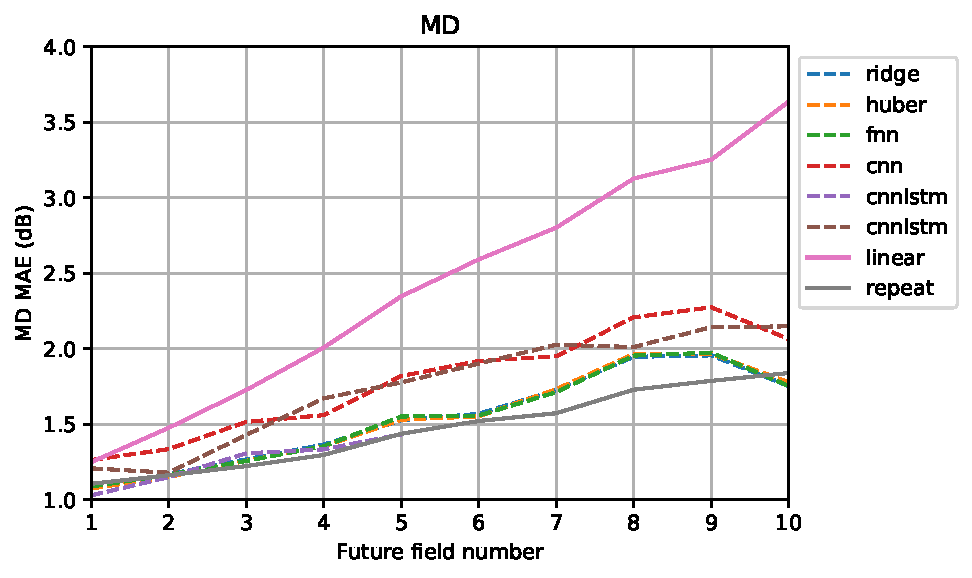
\includegraphics[width=0.8\textwidth]{ml_md.pdf}
		\caption{}
	\end{subfigure}
	\hfill
	\begin{subfigure}[b]{\textwidth}
		\centering
		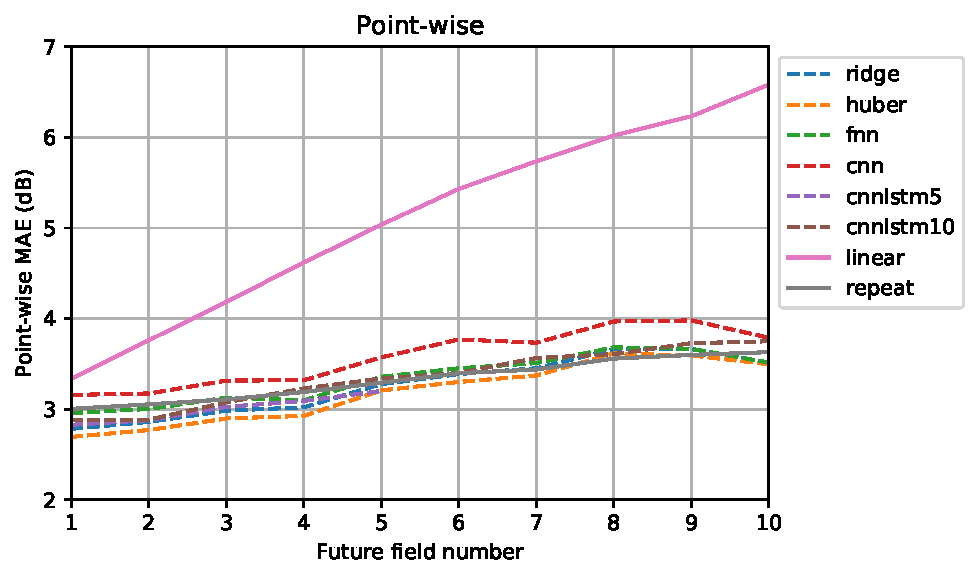
\includegraphics[width=0.8\textwidth]{ml_vf.pdf}
		\caption{}
	\end{subfigure}
	\caption[\acs{MD} and point-wise field prediction results for learning algorithms]{\acs{MD} and point-wise field prediction results for learning algorithms with 3 inputs, compared to the linear extrapolator and repeating the last observed value ``repreat''. There is no significant difference between the learning methods, and due to the dataset containing mostly stable patients, there is no significant difference between the learning methods and ``repeat''. However, all methods performed better than the linear extrapolation methods. }
	\hfill\\
	(In an earlier version of this figure, it was shown that the CNN+LSTM model performed slightly better than other learning methods. This has been corrected in this latest batch of experiments.)
	\label{fig:ml_fig}
\end{figure}

\begin{table}[p]
\centering
\caption{Learning algorithm performance for the 5-th and 10-th prediction}
(25\%/50\%/75\% are the 25-th percentile/median/75-th percentile respectively)
\label{tab:ml_tab}

\hspace*{-1.5cm}
\begin{tabular}{@{}llllllllll@{}}
\toprule
Prediction &      &   \multicolumn{6}{c}{Learning Algorithm} &  \multicolumn{2}{c}{Extrapolation}  \\
\cmidrule(lr){3-8} \cmidrule(lr){9-10}
\acs{MAE} (dB) &      & Ridge & Huber & \acs{MLP}  & \acs{CNN}  & CNN+LSTM5 & CNN+LSTM10 & Linear & Repeat \\ \midrule
& mean & 1.53  & 1.53  & 1.55 & 1.82 & 1.43     & 1.78      & 2.35   & 1.44   \\
MD, & std  & 1.7   & 1.73  & 1.76 & 1.83 & 1.44     & 1.63      & 2.75   & 1.59   \\
5-th& 25\% & 0.45  & 0.45  & 0.44 & 0.59 & 0.49     & 0.59      & 0.64   & 0.43   \\
& 50\% & 1.05  & 1.02  & 1.04 & 1.3  & 1.03     & 1.44      & 1.41   & 0.99   \\
& 75\% & 1.93  & 1.93  & 1.97 & 2.5  & 1.93     & 2.3       & 2.95   & 1.85   \\
\midrule
& mean & 1.75  & 1.78  & 1.75 & 2.06 &          & 2.15      & 3.64   & 1.84   \\
MD, & std  & 1.75  & 1.76  & 1.78 & 2.01 &          & 2.16      & 4.28   & 2.17   \\
10-th & 25\% & 0.57  & 0.6   & 0.57 & 0.64 &          & 0.65      & 0.81   & 0.51   \\
& 50\% & 1.27  & 1.27  & 1.23 & 1.45 &          & 1.47      & 1.91   & 1.18   \\
& 75\% & 2.32  & 2.29  & 2.24 & 2.8  &          & 2.79      & 4.94   & 2.3    \\
\midrule
& mean & 3.28  & 3.21  & 3.36 & 3.57 & 3.2      & 3.34      & 5.04   & 3.29   \\
Point-wise, & std  & 3.55  & 3.63  & 3.85 & 4.08 & 3.69     & 3.87      & 5.85   & 4.18   \\
5-th& 25\% & 0.95  & 0.89  & 0.88 & 0.94 & 1        & 1         & 1      & 1      \\
& 50\% & 2.14  & 2.02  & 2.04 & 2.21 & 1.91     & 1.94      & 3      & 2      \\
& 75\% & 4.25  & 4.1   & 4.27 & 4.53 & 4        & 4.1       & 7      & 4      \\
\midrule
& mean & 3.51  & 3.5   & 3.51 & 3.79 &          & 3.75      & 6.58   & 3.63   \\
Point-wise, & std  & 3.58  & 3.74  & 3.86 & 4.16 &          & 4.33      & 7.39   & 4.6    \\
10-th& 25\% & 1.11  & 1.05  & 1    & 1.03 &          & 1         & 1      & 1      \\
& 50\% & 2.42  & 2.34  & 2.24 & 2.41 &          & 2.21      & 4      & 2      \\
& 75\% & 4.61  & 4.54  & 4.54 & 4.94 &          & 4.64      & 10     & 5      \\ \bottomrule
\end{tabular}
\end{table}

\section{Discussion}



